\chapter{Charge}

If you rub a balloon against your hair, then place it next to a wall, it will stick. This is because it stole some
electrons from your hair, and now the ballon has slightly more
electrons than protons. We say that it has gotten an \textit{electrical charge}. In this case, the balloon has a negative electrical
charge.

Objects with slightly more protons than electrons have a positive charge.

This charge is measured in coulombs. The charge of a single proton is
about $1.6 \times 10^{-19}$ coulombs.

An object with a negative charge and an object with a positive charge
will be attracted to each other. Two objects with the same charge will
be repelled by each other.
% ADD: Good place for culloms law
% KA: https://www.khanacademy.org/science/hs-physics/x215e29cb31244fa1:types-of-interactions/x215e29cb31244fa1:coulomb-s-law/v/coulombs-law

\begin{mdframed}[style=important, frametitle={Coulomb's Law}]\index{Coulomb's law}

  If two objects with charge $q_1$ and $q_2$ (in coulombs) are $r$ meters from each other, the force of attraction or repulsion is given by

  $$F = K\frac{\lvert q_1 q_2 \rvert}{r^2}$$

    where $F$ is in newtons and $K$ is Coulomb's constant: about $8.988 \times 10^9$.
  
\end{mdframed}


\begin{Exercise}[title={Coulomb's Law}, label=charged_balloons]

Two balloons are charged with an identical quantity and type of
charge: $-5 \times 10^{-9}$ coulombs. They are held apart at a
separation distance of 12 cm. Determine the magnitude of the
electrical force of repulsion between them. 
  
\end{Exercise}
\begin{Answer}[ref=charged_balloons]

  $$F = K\frac{\lvert q_1 q_2 \rvert}{r^2} = (8.988 \times 10^9) \frac{(-5 \times 10^{-9})(-5 \times 10^{-9})}{0.12^2} = \frac{224.7 \times 10^{-9}}{0.0144} = 15.6 \times 10^{-6}$$

  15.6 micronewtons.
  
\end{Answer}

At this point, you might ask ``If the wall has zero
charge, why is the balloon attracted to it?'' The answer: the
electrons in the wall move away from the balloon. The negative charge
on the balloon pushes electrons into the wall, so the surface of the
wall gets a mild positive charge. The surface is close to the balloon,
so the attraction is stronger than the repulsion.

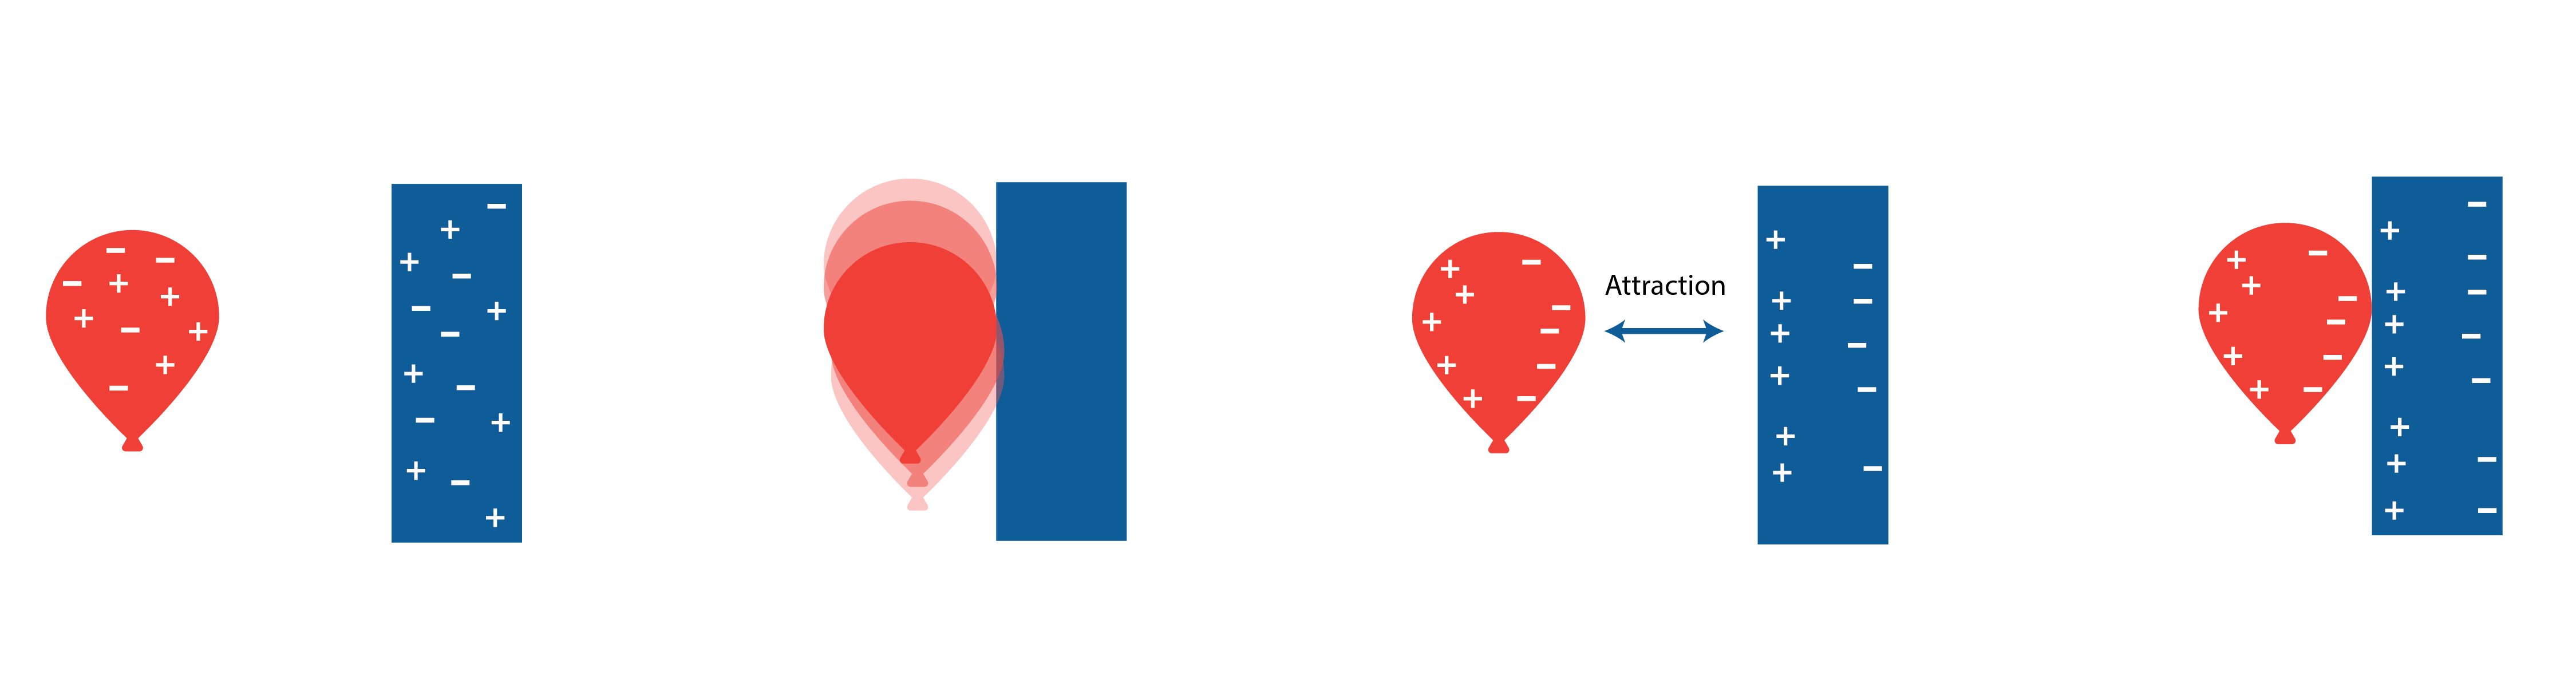
\includegraphics[width=1\textwidth]{balloon2.png}

\section{Lightning}

A cloud is a cluster of water droplets and ice particles. These
droplets and ice particles are always moving up and down through the
cloud. In this process, electrons get stripped off and end up on the
water droplets at the bottom of the cloud (water droplets collect at the bottom because they are denser). The air between the
droplets is a pretty good insulator, which means the electrons are reluctant
to jump anywhere. However, eventually, the charge gets so strong that
even the insulating properties of the air is not enough to prevent
the jump, causing lightning.
% ADD: Add water density explanation. ice less dense than liquid water due to crystaline structure.

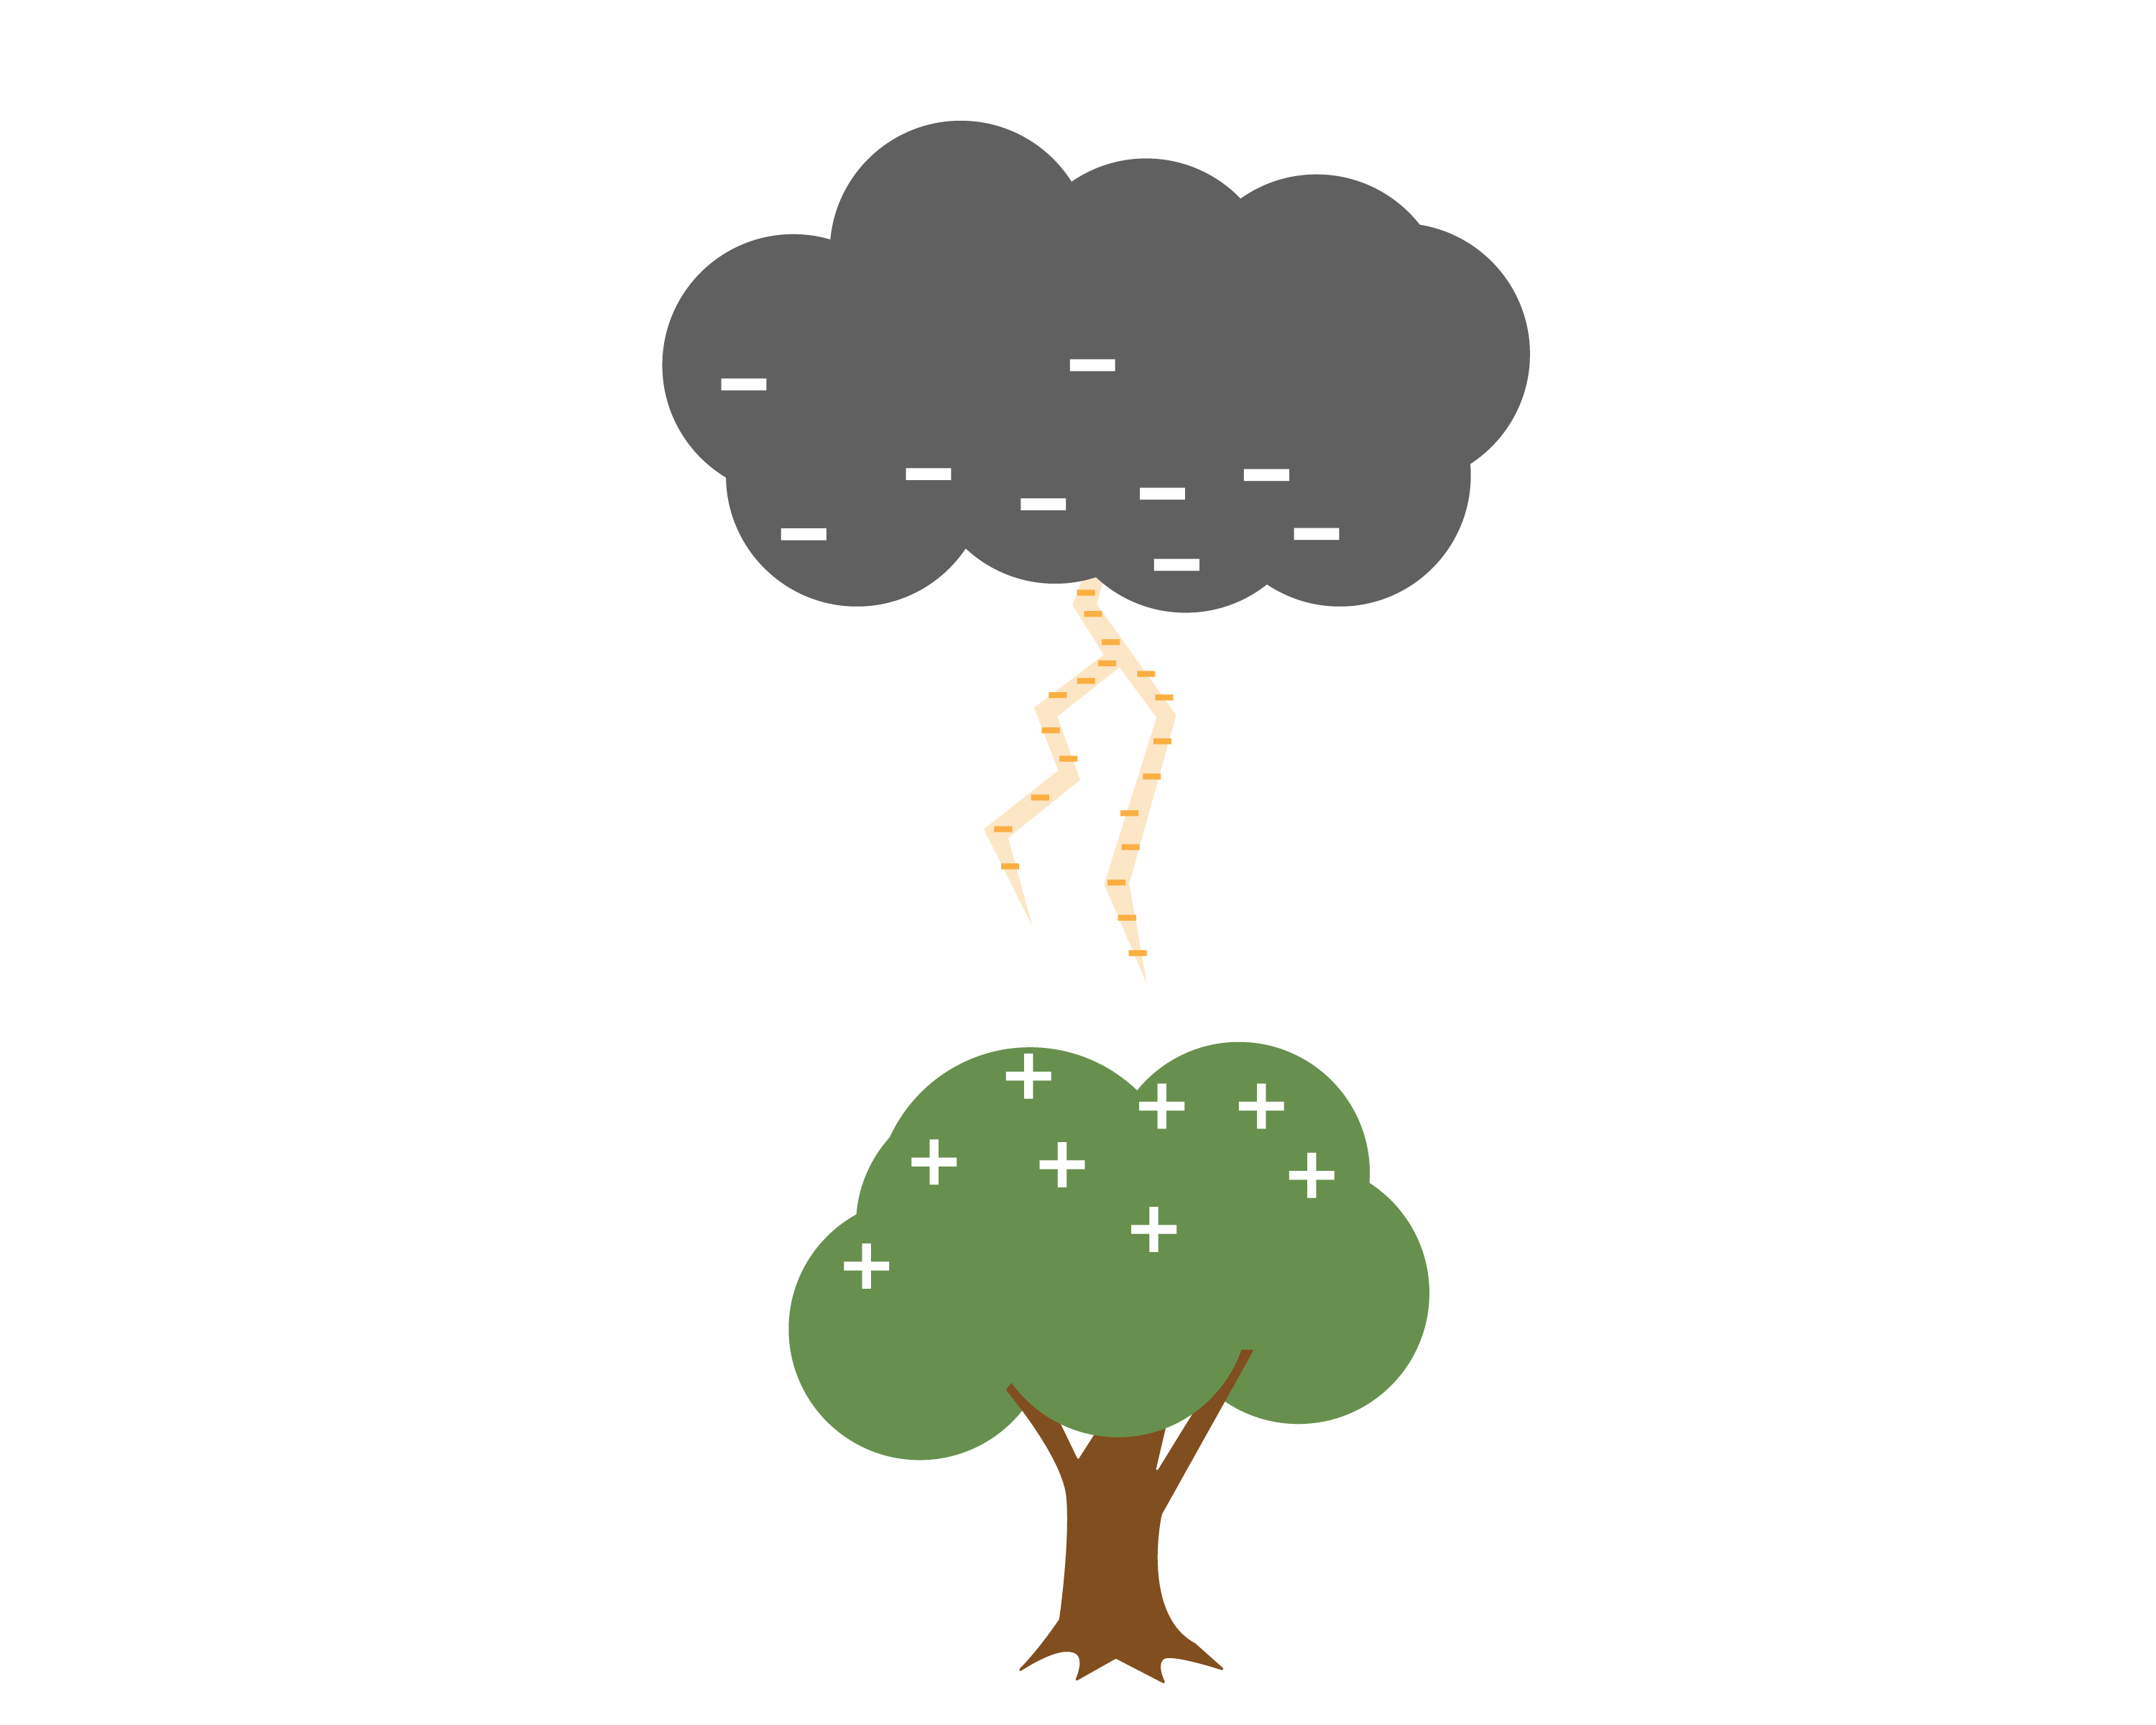
\includegraphics[width=1\textwidth]{lightning.png}

A great deal of lightning moves within a cloud or between clouds. However, sometimes it jumps to the earth. These bolts of lightning vary in the amount of
electrons they carry, but the average is about 15 coulombs.

Thunder occurs because the electrons heat the air they pass through, 
causing the air to expand suddenly. Tthe resulting shockwave is the sound we know as thunder.
% ADD: Relate speed of light and sound 
\section{But...}

This idea that opposite charges attract creates some heavy questions
that you do not yet have the tools to work with. So to these questions, the answer is
basically ``Don't ask that yet!''

However, you probably have these questions, so we will point you in
the direction of the answers.

The first is ``In any atom bigger than hydrogen, there are multiple
protons in the nucleus. Why don't the protons push each other out of
the nucleus?''

We aren't ready to talk about it, but there is a force called \textit{the
 nuclear force}, which pulls the protons and neutrons in the nucleus
of the atom toward each other. At very, very small distances, it is
strong enough to overpower the repulsive force due to the protons'
charges.
% ADD: Effective nuclear charge

Another question is ``Why do the electrons whiz around in a cloud so
far from the nucleus of the atom? Negatively charged electrons should
cling to the protons in the center, right?''

We aren't ready to talk about this either, but quantum mechanics tells us that
electrons like to live in a certain specific energy level. Hugging
protons isn't one of those levels.
